\documentclass[a4paper,11pt]{article}
\usepackage{graphicx}
\usepackage[margin=1in]{geometry}

\usepackage[table,xcdraw]{xcolor}
\usepackage[utf8]{inputenc}
\usepackage{ulem}
\usepackage{color}
\usepackage{enumerate}
\usepackage{amssymb}
\usepackage{amsmath}
\usepackage {tikz}
\usetikzlibrary{arrows,matrix,positioning,fit}
%\usepackage{bera}
\usepackage{listings}
\usepackage{xcolor}
\usepackage{framed}
\usepackage[hidelinks]{hyperref}
\usepackage{enumitem}
%\setenumerate[2]{label=\roman*.}
\usepackage{blindtext}
\usepackage{fancyhdr}
\pagestyle{fancy}
\usepackage{hhline}
\colorlet{punct}{red!60!black}
\definecolor{background}{HTML}{EEEEEE}
\definecolor{delim}{RGB}{20,105,176}
\colorlet{numb}{magenta!60!black}

\definecolor {processblue}{cmyk}{0.96,0,0,0}

%\setenumerate[1]{label=\textbf{\thesection.\arabic*.}}


\begin{document}
\textbf{Integration of 1-forms on Graphs}

\bigskip

\textbf{Introduction}

\bigskip

Given a connected graph $G=(V,E)$ with $V$ vertices, and $E$ edges and a 
1-form $v: E \rightarrow \mathbb{R}^D$. We're looking for the 0-form 
$x: V \rightarrow \mathbb{R}^D$ minimizing the error:

$$E(x) = \sum_{(i,j) \in E} ||dx_{ij} - v_{ij}||^2$$

where $dx: E \rightarrow \mathbb{R}^D$ is the differential of $x$.

\bigskip

\textbf{Obs. 1}: It is sufficient to consider the case $D=1$, because 
the problem can be reduced to solving $D$ independent 1-D problems on 
the same graph for each coordinate.

\bigskip

\textbf{Obs. 2} (Abuses of notation): We use $V$ to denote both the set 
of vertices and the total number of vertices of the graph. And we denote 
$v$ to the 1-form and $v_i$ is the $i-th$ vertex.

\bigskip

\textbf{Obs. 3}: Vertices and edges can be enumerated in many different 
ways. We will enumerate vertices and edges according to a traversal 
order of a spanning tree. This process determines a consistent 
orientation of the edges: an edge will be oriented from a lower vertex 
to a greater vertex:

$$e_{ij}: v_i \rightarrow v_j \ (for \ i < j)$$

\bigskip

\textbf{Integration process}

\bigskip

The proposed process for integrating $v$ is as follows:

\begin{enumerate}
	\item Construct a spanning tree $T$ for $G$
	\item Choose an order of traversal for $T$ and orient the edges 
	from parent to child
	\item Enumerate the vertices and tree edges according to the order 
	of traversal (See figure~\ref{fig:M1})
	\item We will refer to the remaining graph edges (those which do not 
	belong to the tree) as ``loop-edges". Orient the loop-edges from 
	parent to child.
	\item Construct the oriented incidence matrix $D$: this is an $E \times V$ 
	sparse matrix with one row per graph edge and one column per vertex. 
	For each edge $e_{ij} \ (i < j)$ we set the $i-th$ column entry to $-1$ 
	and the $j-th$ column to $1$. Rows representing tree-edges come first 
	and are ordered such that the $N-1 \times N-1$ upper-right submatrix 
	is lower triangular (See figure~\ref{fig:M2}).
	\item Solve the linear system $D^tDx=D^tv$ (see below).
\end{enumerate}


\begin{figure}
\centering
\begin {tikzpicture}[-latex ,auto ,node distance =3cm ,on grid ,
semithick ,state/.style ={ circle ,top color =white , bottom color = processblue!20 ,
draw,processblue , text=blue , minimum width =1 cm},
edge/.style = {->,> = latex'}]
\node[state] (1) {$1$};
\node[state] (2) [below left=of 1] {$2$};
\node[state] (3) [below  right =of 1] {$3$};
\node[state] (4) [below  left =of 2] {$4$};
\node[state] (5) [below  left =of 3] {$5$};
\node[state] (6) [below  right =of 3] {$6$};
\node[state] (7) [below  left =of 4] {$7$};
\node[state] (8) [below  right =of 4] {$8$};
\node[state] (9) [below  right =of 5] {$9$};
\path (1) edge node {1} (2);
\path (1) edge node {2} (3);
\path (2) edge node {3} (4);
\path (3) edge node {4} (5);
\path (3) edge node {5} (6);
\path (4) edge[red] node {} (5);
\path (4) edge node {6} (7);
\path (4) edge node {7} (8);
\path (5) edge node {8} (9);
\path (8) edge[red] node {} (9);
\end{tikzpicture}

\caption{BFS traversal of a spanning tree. Nodes and edges are 
enumerated according to tree traversal. Edges are oriented from 
parent to child. Red edges correspond to 
$loop-edges$.}
\label{fig:M1}
\end{figure}

\begin{figure}
\centering
%$\begin{pmatrix}
%-1 & 1  & 0  & 0  & 0  & 0 & 0 & 0  & 0 &  \\
%-1 & 0  & 1  & 0  & 0  & 0 & 0 & 0  & 0 &  \\
%0  & -1 & 0  & 1  & 0  & 0 & 0 & 0  & 0 &  \\
%0  & 0  & -1 & 0  & 1  & 0 & 0 & 0  & 0 &  \\
%0  & 0  & -1 & 0  & 0  & 1 & 0 & 0  & 0 &  \\
%0  & 0  & 0  & -1 & 0  & 0 & 1 & 0  & 0 &  \\
%0  & 0  & 0  & -1 & 0  & 0 & 0 & 1  & 0 &  \\
%0  & 0  & 0  & 0  & -1 & 0 & 0 & 0  & 1 &  \\
%0  & 0  & 0  & -1 & 1  & 0 & 0 & 0  & 0 &  \\
%0  & 0  & 0  & 0  & 0  & 0 & 0 & -1 & 1 &
%\end{pmatrix}$
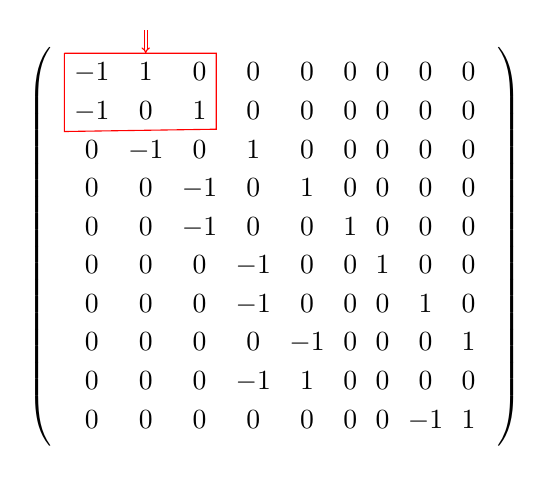
\begin{tikzpicture}
	\matrix [matrix of math nodes,left delimiter=(,right delimiter=)] (m)
	{
		-1 & 1  & 0  & 0  & 0  & 0 & 0 & 0  & 0 &  \\
		-1 & 0  & 1  & 0  & 0  & 0 & 0 & 0  & 0 &  \\
		0  & -1 & 0  & 1  & 0  & 0 & 0 & 0  & 0 &  \\
		0  & 0  & -1 & 0  & 1  & 0 & 0 & 0  & 0 &  \\
		0  & 0  & -1 & 0  & 0  & 1 & 0 & 0  & 0 &  \\
		0  & 0  & 0  & -1 & 0  & 0 & 1 & 0  & 0 &  \\
		0  & 0  & 0  & -1 & 0  & 0 & 0 & 1  & 0 &  \\
		0  & 0  & 0  & 0  & -1 & 0 & 0 & 0  & 1 &  \\
		0  & 0  & 0  & -1 & 1  & 0 & 0 & 0  & 0 &  \\
		0  & 0  & 0  & 0  & 0  & 0 & 0 & -1 & 1 &  \\
	};  
	\draw[color=red] (m-1-1.north west) -- (m-1-3.north east) -- (m-2-3.south east) -- (m-2-1.south west) -- (m-1-1.north west);
	\draw[color=red,double,implies-](m-1-2.north) -- +(0,0.3);
\end{tikzpicture}

\caption{Incidence matrix correspondig to graph in figure~\ref{fig:M1}. 
The first column corresponds to the tree root, it can be dropped. 
Green and blue submatrices correspond to tree-edges and loop-edges, 
respectively. The tree-edge submatrix is lower triangular.}
\label{fig:M2}
\end{figure}

\newpage

\textbf{Properties of the oriented incidence matrix $D$ and other facts}

\bigskip

\underline{Dropping the root column of $D$}

\bigskip

We can rewrite the minimization problem in matrix form as follows:

$$E(x) = \sum_{(i,j) \in E} ||dx_{ij} - v_{ij}||^2 = || D x - v||^2$$

Note that as we are dealing with an integration problem, the solutions 
are equivalent \textit{modulo a translation}. The consequence of this 
fact is that we can fix the value of the tree root (ie. $x_1 = 0$). 
Thus we can drop the first column of $D$. (See 
figure~\ref{fig:M2})

\bigskip

\underline{Relation to the \textit{Laplacian} matrix and rank of $D$}

\bigskip

The directed incidence matrix has the following property:

$$L = D^t D$$

where $L$ is the \textit{Laplacian} matrix of $G$. The rank of 
$L$ is: $n-c$ (where $c$ is the number of connected components of $G$). 
In our case, as $G$ is connected, the rank of $L$ (and consequently the 
rank of $D$) is $n-1$.

\bigskip

\underline{The problem is equivalent to solve a linear system}

\bigskip

To solve the minimizatiom problem is equivalent to find where the 
gradient of $E(x)$ vanishes:
 
$$\nabla E = [\frac{\partial E}{\partial x_1}, \dots, \frac{\partial 
E}{\partial x_n}] = D^tDx-D^tv=0$$

It is equivalent to solve the linear system:

$$D^tDx = D^tv$$

As the rank of $D$ is $n-1$, the linear system may not have a solution. 
But solving the problem by iterative methods will converge to the 
closest ``possible" guess.

\bigskip

\underline{The full rank matrix $M$ based on $D$}

\bigskip

A full rank $E \times E$ matrix can be constructed based on $D$. We 
drop the first column of $D$ (as pointed before) to obtain $D'$ (a $E 
\times (V-1)$ matrix). Suppose that we rewrite $D'$ as follows:

\begin{equation}
     D'=\begin{bmatrix}
         T \\
         L
	\end{bmatrix}
 \end{equation}

Where the rows of $T$ correspond to tree edges and the rows of $L$ to 
loop-edges. We can append $E-V+1$ linearly independent columns 
spannning the orthogonal complement of $D'$:

\begin{equation}
     D'=\begin{bmatrix}
         T B\\
         L I
	\end{bmatrix}
\end{equation}

Where $I$ is the indentity matrix and the following orthogonality 
condition is satisfied: 

\begin{equation}
     0=\begin{bmatrix}
         T \\
         L
	\end{bmatrix}^t
	\begin{bmatrix}
         B\\
         I
	\end{bmatrix}
\end{equation}

This implies that

$$B = -(L)^{-t}A^t$$

The minimization we are intended to solve is equivalent to solve this 
linear system:

\begin{equation}
     M \begin{bmatrix}
         x \\
         y
	\end{bmatrix}=\begin{bmatrix}
         T B\\
         L I
	\end{bmatrix}
	\begin{bmatrix}
         x \\
         y
	\end{bmatrix} = v
\end{equation}

Where $[x\ y]^t \in \mathbb{R}^E$.

\bigskip

\underline{The columns of the $B$ matrix}

\bigskip

As described in the last part, the $B$ matrix is defined in terms of an 
orthogonality condition. This definition is not practical for 
computation purposes, because of the inverse ($L^{-t}$). Another 
definition can be given (OBS: have to demonstrate equivalence!).

\bigskip

The definition is as follows:

\begin{itemize}
	\item Every loop-edge $e_{ij}=(v_i, v_j)$ induces a cycle in the 
	spanning tree.
	\item The directed paths $p_{i,root}=(v_i, v_{root})$ and $p_{j,root}=(v_j, 
	v_{root})$, have a first common vertex namely $v_k$ (See 
	figure~\ref{fig:M3}).
	\item The column in $B$ associated to the loop-edge $e_{ij}$, must 
	set the rows (tree-edges) of the path $p_{i,k}=(v_i, v_k)$ to $1$ and the rows 
	(tree-edges) of the path $p_{j,k}=(v_j, v_k)$ to $-1$ (See 
	figure~\ref{fig:M3}).
\end{itemize}

\underline{Two different linear systems solve the problem}

\bigskip

As pointed previously there are two linear systems that solve the 
integration problem:

\begin{equation}
     M \begin{bmatrix}
         x \\
         y
	\end{bmatrix}=v
\end{equation}

And:

$$D^tDx = D^tv$$

Intuitively the second version seems easier to solve because $D^tD$ is 
a Laplacian matrix which is well conditioned, while $M$ is not even 
sparse. Nevertheless the columns of $M$ can be computed on demand in 
each iteration of an iterative solver. So some solid experiments should 
be carried to prove this intuition.

\newpage

\begin{figure}
\centering
\begin {tikzpicture}[-latex ,auto ,node distance =3cm ,on grid ,
semithick ,state/.style ={ circle ,top color =white , bottom color = processblue!20 ,
draw,processblue , text=blue , minimum width =1 cm}]
\node[state] (1) {$root$};
\node[state] (2) [below =of 1] {$k$};
\node[state] (3) [below  left =of 2] {$i$};
\node[state] (4) [below  right =of 2] {$j$};
\draw[dashed] (1) .. controls (1,-1) and (-1,-2) .. (2);
\draw[dashed] (2) .. controls (-2,-3) and (0,-4) .. (3);
\draw[dashed] (2) .. controls (2,-3) and (0,-4) .. (4);
\draw[red] (3) -- (4);
\end{tikzpicture}

%\begin{tikzpicture}[-latex ,auto ,node distance =3cm ,on grid ,
%semithick ,state/.style ={ circle ,top color =white , bottom color = processblue!20 ,
%draw,processblue , text=blue , minimum width =1 cm},edge from parent path=
%{(\tikzparentnode.south) .. controls +(0,-2) and +(0,2) .. (\tikzchildnode.north)}]
%\node[state] {root}
	%child[state] {node {left}}	
	%child[state] {node {right}
		%child[state] {node {child}}
		%child[state] {node {child}}
	%};
%\end{tikzpicture}

\caption{The red coloured loop-edge induces a cycle in the spanning 
tree. Node $v_k$ is the first common node in the paths $p_{i,root}$ 
and $p_{j,root}$.}
\label{fig:M3}
\end{figure}


\begin{figure}
\centering
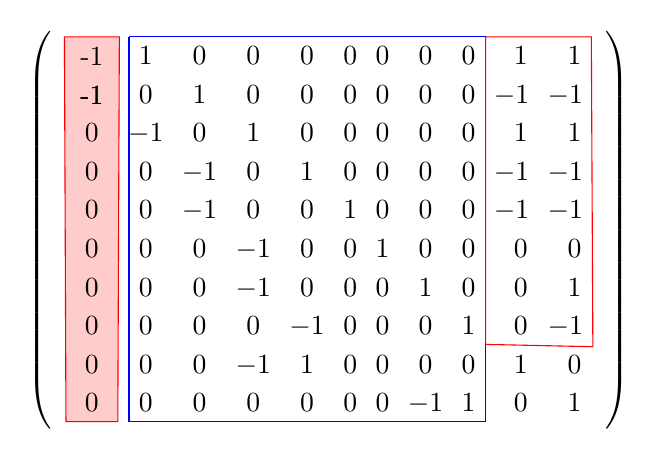
\begin{tikzpicture}
	\matrix [matrix of math nodes,left delimiter=(,right delimiter=)] (m)
	{
		-1 & 1  & 0  & 0  & 0  & 0 & 0 & 0  & 0 & \ \ 1 & \ \ 1 &  \\
		-1 & 0  & 1  & 0  & 0  & 0 & 0 & 0  & 0 & -1 & -1 &  \\
		\ \ 0& -1 & 0  & 1  & 0  & 0 & 0 & 0  & 0 & \ \ 1 & \ \ 1 &  \\
		\ \ 0& 0  & -1 & 0  & 1  & 0 & 0 & 0  & 0 & -1 & -1 &  \\
		\ \ 0& 0  & -1 & 0  & 0  & 1 & 0 & 0  & 0 & -1 & -1 &  \\
		\ \ 0& 0  & 0  & -1 & 0  & 0 & 1 & 0  & 0 & \ \ 0  &  \ \ 0 &  \\
		\ \ 0& 0  & 0  & -1 & 0  & 0 & 0 & 1  & 0 & \ \ 0  &  \ \ 1 &  \\
		\ \ 0& 0  & 0  & 0  & -1 & 0 & 0 & 0  & 1 & \ \ 0  & -1 &  \\
		\ \ 0& 0  & 0  & -1 & 1  & 0 & 0 & 0  & 0 & \ \ 1  &  \ \ 0 &  \\
		\ \ 0& 0  & 0  & 0  & 0  & 0 & 0 & -1 & 1 & \ \ 0  & \ \ 1 &  \\
	}; 
	\draw[color=blue] (m-1-2.north west) -- (m-1-9.north east) -- 
	(m-10-9.south east) -- (m-10-2.south west) -- (m-1-2.north west);

	\draw[color=red] (m-1-10.north west) -- (m-1-11.north east) -- 
	(m-8-11.south east) -- (m-8-10.south west) -- (m-1-10.north west);

	\draw[color=red, fill=red!20] (m-1-1.north west) -- (m-1-1.north east) -- 
	(m-10-1.south east) -- (m-10-1.south west) -- (m-1-1.north west);
	\foreach \Pos/\Nodo in 
	{m-1-1/-1,m-2-1/-1,m-2-1/-1,m-3-1/0,m-4-1/0,m-5-1/0,m-6-1/0,m-7-1/0,m-8-1/0,m-9-1/0,m-10-1/0}
		\node at (\Pos) {\Nodo};

\end{tikzpicture}

\caption{Full-rank matrix correspondig to graph in figure~\ref{fig:M1}. 
The first column corresponds to the tree root, it can be dropped. 
Blue and red submatrices correspond to $D'$ and $B$, 
respectively.}
\label{fig:M4}
\end{figure}

\newpage

\textbf{Laplace and Poisson Problems}

\bigskip

The $Laplace \ operator$ $\Delta$ is a differential operator, namely the divergence 
of the gradient of a function $f$. Locally, $\Delta f(p)$ it is the rate at which the 
average value of $f$ over spheres centered at $p$ deviates from $f(p)$ 
as the radius of the spheres grow. In 3-space $Cartesian \  
coordinates$ it can be expressed in the following terms:

$$\Delta f = \frac{\partial^2 f}{\partial^2 x}+\frac{\partial^2 f}{\partial^2 
y}+\frac{\partial^2 f}{\partial^2 z}$$

\bigskip

The $Laplace \ equation$ is the following differential equation:

$$\Delta f = 0$$

A natural motivation for the Laplacian equation arises in the theory of 
diffusion. Specifically, if $u$ is the density at equilibrium of a 
chemical concentration, then the net flux of $u$ through the boundary 
of any smooth region $V$ is zero (provided there is no source or sink 
within $V$):

$$\int_{\partial V} \nabla u \centerdot n \ dS = 0$$

where $n$ is the outward unit normal to the boundary of $V$.

\bigskip

A very similar equation is $Poisson's \ equation$:

$$\Delta \phi = f$$

\emph{Surface reconstruction}

\bigskip 

Among other applications, this equation can be used to reconstruct a 3D 
surface based on a (large) set of points $p_i$ where each point also 
carries an estimate of the local surface normal $n_i$.

\bigskip

This technique reconstructs the implicit function $f$ whose value is 
zero at the points $p_i$ and whose gradient at those points equals the 
normal vectors $n_i$. The set $(p_i, n_i)$ is a sampling of a 
continuous vector field $V$. The implicit function $f$ is found by 
integrating the vector field. Since not every vector field is the 
gradient of a function, the problem may not have a solution. The 
neccessary and sufficient condition for a smooth vector field $V$ to be 
the gradient of a function $f$ is that the $curl$ of $V$ must be 
identically zero. It is still possible to perform a $least-squares$ fit 
to minimize the difference between $V$ and the gradient of $f$. (see 
Taubin and Calakli paper)

\bigskip

\emph{Discrete formulations of Laplace and Poisson operators}

\bigskip

Among the different formulations of the discrete Laplace operator, two 
are of interest in this context: Graph Laplacians and Mesh Laplacians.

\bigskip

\textit{Graph Laplacians}

\bigskip

Let $G=(V,E)$ be a graph, and let $\phi: V \rightarrow R$ be a function 
of the vertices taking values in a ring (ie $\mathbb{Z}$, $\mathbb{R}$). 
Then the \textit{discrete Laplacian} $\Delta$ acting on $\phi$ is defined by

$$(\Delta \phi)(v) = \sum_{w \in N(v)} [\phi(v) - \phi(w)]$$

where $N(v)$ are the neighbors of the vertex $v \in V$. This definition 
clarifies the definition of the $Laplacian \ matrix$ associated to a 
graph. The latter is just the discrete Laplacian expressed in matrix 
form.

\bigskip

If the graph has weighted edges, that is, a weighting function $\gamma: 
E \rightarrow R$ is given, then the definition can be generalized to:

$$(\Delta_{\gamma} \phi)(v) = \sum_{w \in N(v)} \gamma_{vw} [\phi(v) - \phi(w)]$$

where $\gamma_{wv}$ is the weight value on the edge $(v,w) \in E$

\bigskip

Closely related to the discrete Laplacian is the \textit{averaging 
operator}:

$$(M \phi)(v) = \frac{1}{deg \ v} \sum_{w \in N(v)} \phi(w)$$

\textit{Mesh Laplacians}

\bigskip

\textit{Mesh Laplace operators} take into account the geometry of  a 
surface (e.g. the angles at the nodes). (see Reuter, Biasotti, Giorgi, 
Patane, Spagnuolo: Discrete Laplace-Beltrami operators for shape 
analysis and segmentation)

\newpage

\textbf{Finding the best spanning tree}

\bigskip

The election of the initial spanning tree determines the solution of 
the problem.

\smallskip

Finding the best initial spanning tree seems to be a difficult task. 
Algorithms to find all the spanning trees of a graph (see Tarjan, Matsui).

\bigskip

\underline{A simple example}

\bigskip

More precisely different spanning trees induce different solutions. 
Consider the following weighted triangle graph:

\bigskip

\begin {tikzpicture}[-latex ,auto ,node distance =3cm,on grid,
semithick ,state/.style ={ circle ,top color =white , bottom color = processblue!20,
draw,processblue , text=blue , minimum width =1 cm},edge/.style = {->,> = stealth'}]
\node[state] (1) {$1$};
\node[state] (2) [below left=of 1] {$2$};
\node[state] (3) [below  right =of 1] {$3$};
\draw (1) edge[-] node {1000} (2);
\path (1) edge[-] node {30} (3);
\path (2) edge[-] node {5} (3);
\end{tikzpicture}

Lets analyze the six directed spanning trees:

\begin{itemize}
	\item $T_1=(v_1,e_{23})$
	\item $T_2=(v_1,e_{32})$
	\item $T_3=(v_2,e_{13})$
	\item $T_4=(v_2,e_{31})$
	\item $T_5=(v_3,e_{12})$
	\item $T_6=(v_3,e_{21})$
\end{itemize}

Where the tree $T_i = (v,e_{ij})$ has $v$ as root and the directed edge 
$e_{ij} = (v_i \rightarrow v_j)$ is the induced loop edge. To compare 
the solutions we first solve the linear system associated to each tree: 

\begin{equation}
     M \begin{bmatrix}
         x \\
         y
	\end{bmatrix}=\begin{bmatrix}
         T B\\
         L I
	\end{bmatrix}
	\begin{bmatrix}
         x \\
         y
	\end{bmatrix} = v
\end{equation}

And then compare the norm of the trees:

$$n = ||v-D'x||_2$$

The results are as follows:

\begin{itemize}
	\item $n_1=562.92$
	\item $n_2=557.14$
	\item $n_3=591.78$
	\item $n_4=557.14$
	\item $n_5=562.92$
	\item $n_6=591.78$
\end{itemize}

\bigskip

\underline{Exact and metaheuristic approaches}

\bigskip

The exact approach finds the best solution. The algorithms are not 
suitable for big datasets. But they may be the best choice for small 
ones.

\bigskip

The metaheuristic approach tries to find good solutions (not 
necessarilly the best) in polynomial time. Some metaheuristics are:

\begin{itemize}
	\item Simulated-annealing
	\item Tabu-search
	\item GRASP
	\item Genetic algorithms
	\item Ant-colony
\end{itemize}

Finding the best metaheuristic depends on the problem and must be 
demonstrated empirically.

\newpage


TODO:

1) Buscar instancias chicas de mallas triangulares para probar en 
octave

Tengo que entender la matriz B del apunte de Gabriel.

Otras partes:

- Descripción del problema de Poisson y Laplace
\end{document}
